\begin{tomtat}
	\begin{minipage}[t]{0.3\textwidth}
		\vspace{0pt}
		\begin{tomtat}
			\begin{center}
				\textbf{ĐỀ 15}
			\end{center}
			
		\end{tomtat}
	\end{minipage}
	\hfill
	\begin{minipage}[t]{0.5\textwidth}
		\vspace{0pt}
		\begin{tomtat}
			\begin{center}
				\includegraphics[scale=0.08]{images/15}
			\end{center}
		\end{tomtat}
	\end{minipage}
\end{tomtat}
\textbf{I. PHẦN TRẮC NGHIỆM}
\begin{ex} % Câu 1
	Biết đồ thị hàm số $y=ax^2$ đi qua điểm $A(-2;4)$. Tìm a?
	\choice{$a=-2$}{$a=4$}{$a=1$}{$a=-1$}
	\loigiai{
		Đồ thị hàm số $y=ax^2$ đi qua điểm $A(-2;4)$ có nghĩa là khi $x=-2$ thì $y=4$.
		Thay $x=-2$ và $y=4$ vào phương trình hàm số, ta được:
		\begin{align*}
			4 &= a(-2)^2 \\
			4 &= a \cdot 4 \\
			a &= \frac{4}{4} \\
			a &= 1
		\end{align*}
		Vậy giá trị của $a$ là 1.
		\\ \textbf{ĐÁP ÁN C}
	}
\end{ex}

\begin{ex} % Câu 2
	Tìm giá trị của $x$ thỏa mãn $(x-1)(2x+3)=0$.
	\choice{$x=1; x=\frac{3}{2}$}{$x=-1; x=\frac{3}{2}$}{$x=1; x=-\frac{3}{2}$}{$x=-1; x=-\frac{3}{2}$}
	\loigiai{
		Ta có phương trình tích $(x-1)(2x+3)=0$.
		Điều này xảy ra khi một trong hai thừa số bằng 0:
		\begin{itemize}
			\item $x-1=0 \Rightarrow x=1$
			\item $2x+3=0 \Rightarrow 2x=-3 \Rightarrow x=-\frac{3}{2}$
		\end{itemize}
		Vậy nghiệm của phương trình là $x=1$ và $x=-\frac{3}{2}$.
		\\ \textbf{ĐÁP ÁN C}
	}
\end{ex}

\begin{ex} % Câu 3
	Các tia nắng mặt trời tạo với mặt đất một góc $60^\circ$ và bóng của một tòa tháp trên mặt đất dài 20m. Tính chiều cao của tòa tháp? (làm tròn đến m)
	\choice{17m}{10m}{35m}{40m}
	\loigiai{
		Gọi $h$ là chiều cao của tòa tháp (cạnh đối) và $b = 20 \text{ m}$ là độ dài bóng trên mặt đất (cạnh kề).
		Góc tạo bởi tia nắng mặt trời và mặt đất là $\alpha = 60^\circ$.
		Ta có mối quan hệ: $\tan \alpha = \frac{\text{cạnh đối}}{\text{cạnh kề}} = \frac{h}{b}$.
		Do đó, $h = b \cdot \tan \alpha$.
		$$ h = 20 \cdot \tan(60^\circ) $$
		Sử dụng máy tính: $\tan(60^\circ) = \sqrt{3} \approx 1,732$.
		$$ h \approx 20 \cdot 1,732 \approx 34,64 \text{ m} $$
		Làm tròn đến mét, ta được $h \approx 35 \text{ m}$.
		\\ \textbf{ĐÁP ÁN C}
	}
\end{ex}

\begin{ex} % Câu 4
	Thể tích V một hình trụ có đường kính đáy bằng 4cm và chiều cao 3cm. (Tính theo $\pi$) là:
	\choice{$12\pi \text{ cm}^3$}{$48\pi \text{ cm}^3$}{$7\pi \text{ cm}^3$}{$37,68\text{cm}^3$}
	\loigiai{
		Đường kính đáy của hình trụ là $d = 4 \text{ cm}$, vậy bán kính đáy là $R = \frac{d}{2} = \frac{4}{2} = 2 \text{ cm}$.
		Chiều cao của hình trụ là $h = 3 \text{ cm}$.
		Thể tích của hình trụ được tính bằng công thức: $V = \pi R^2 h$.
		\begin{align*}
			V &= \pi (2)^2 \cdot 3 \\
			&= \pi \cdot 4 \cdot 3 \\
			&= 12\pi (\text{cm}^3)
		\end{align*}
		\\ \textbf{ĐÁP ÁN A}
	}
\end{ex}

\begin{ex} % Câu 5
	Cho đường tròn tâm O. Hai điểm B, C phân biệt thuộc đường tròn (O), sao cho $\widehat{BOC} = 90^\circ$, tính độ dài cung BC? Biết bán kính đường tròn bằng 4cm, lấy $\pi \approx 3,14$ và kết quả lấy đến hàng phần mười. Kết quả là:
	\choice{6,3cm}{6,2cm}{6cm}{6,28cm}
	\loigiai{
		Độ dài cung tròn được tính bằng công thức: $l = \frac{\pi R n}{180}$.
		Trong đó $R$ là bán kính đường tròn ($R=4 \text{ cm}$) và $n$ là số đo góc ở tâm chắn cung đó ($n=90^\circ$).
		Sử dụng $\pi \approx 3,14$.
		\begin{align*}
			l_{BC} &= \frac{3,14 \cdot 4 \cdot 90}{180} \\
			&= \frac{3,14 \cdot 4 \cdot 1}{2} \\
			&= 3,14 \cdot 2 \\
			&= 6,28 \text{ cm}
		\end{align*}
		Làm tròn kết quả đến hàng phần mười, ta được $6,3 \text{ cm}$.
		(Nếu không làm tròn sớm $\pi$, $l = \frac{4 \cdot 90}{180}\pi = 2\pi \approx 2 \times 3,14159... \approx 6,283... \text{ cm}$, làm tròn đến hàng phần mười là $6,3 \text{ cm}$).
		\\ \textbf{ĐÁP ÁN A}
	}
\end{ex}

\begin{ex} % Câu 6
	Phúc gieo một con xúc xắc 50 lần và thống kê lại kết quả các lần gieo ở bảng sau:
	\begin{center}
		\begin{tabular}{|l|c|c|c|c|c|c|}
			\hline
			1 chấm & 2 chấm & 3 chấm & 4 chấm \\
			\hline
			8 & 9 & 9 & 5 \\
			\hline
		\end{tabular}
	\end{center}
	Tần số xuất hiện mặt 3 chấm là:
	\choice{5}{6}{50}{9}
	\loigiai{
		Dựa vào bảng thống kê kết quả gieo xúc xắc:
		Khi "Mặt" là "3 chấm", "Số lần xuất hiện" (tần số) tương ứng là 9.
		Vậy tần số xuất hiện mặt 3 chấm là 9.
		\\ \textbf{ĐÁP ÁN D}
	}
\end{ex}
\begin{ex}
	Cho phương trình $2x^2+x-1=0$ có tập nghiệm là:
	\choice{$\{-1; \frac{1}{2}\}$}{$-\frac{1}{2}; 1$}{$\{-1\}$}{$\emptyset$}
	\loigiai{
		Phương trình $2x^2+x-1=0$ là phương trình bậc hai có dạng $ax^2+bx+c=0$ với $a=2$, $b=1$, $c=-1$.
		Ta tính biệt thức $\Delta = b^2-4ac = 1^2 - 4(2)(-1) = 1 + 8 = 9$.
		Vì $\Delta > 0$ nên phương trình có hai nghiệm phân biệt:
		$x_1 = \frac{-b + \sqrt{\Delta}}{2a} = \frac{-1 + \sqrt{9}}{2(2)} = \frac{-1+3}{4} = \frac{2}{4} = \frac{1}{2}$.
		$x_2 = \frac{-b - \sqrt{\Delta}}{2a} = \frac{-1 - \sqrt{9}}{2(2)} = \frac{-1-3}{4} = \frac{-4}{4} = -1$.
		Vậy tập nghiệm của phương trình là $S = \{-1; \frac{1}{2}\}$.\\
		\textbf{ĐÁP ÁN A}
	}
\end{ex}


\begin{ex} % Câu 8
	Cho hình nón có bán kính đáy bằng 5cm, độ dài đường sinh bằng 10 cm. Diện tích xung quanh của hình nón (lấy $\pi \approx 3,14$) là:
	\choice{$157\text{cm}^2$}{$157\text{cm}$}{$15,7\text{cm}$}{$15,7\text{cm}^2$}
	\loigiai{
		Diện tích xung quanh của hình nón được tính bằng công thức: $S_{xq} = \pi Rl$.
		Trong đó:
		$R$ là bán kính đáy của hình nón ($R=5 \text{ cm}$).
		$l$ là độ dài đường sinh của hình nón ($l=10 \text{ cm}$).
		Sử dụng $\pi \approx 3,14$.
		\begin{align*}
			S_{xq} &= \pi \cdot R \cdot l \\
			&= 3,14 \cdot 5 \cdot 10 \\
			&= 3,14 \cdot 50 \\
			&= 157 (\text{cm}^2)
		\end{align*}
		\\ \textbf{ĐÁP ÁN A}
	}
\end{ex}
\textbf{II. PHẦN TỰ LUẬN}
\begin{ex} % Câu 9
	Rút gọn biểu thức: $A = \left(\frac{1}{x-2\sqrt{x}} + \frac{1}{\sqrt{x}-2}\right) : \frac{\sqrt{x}+1}{x-4\sqrt{x}+4}$ (với $x>0; x \ne 4$).
	\loigiai{
		Với $x>0; x \ne 4$, ta có:
		$x-2\sqrt{x} = \sqrt{x}(\sqrt{x}-2)$.
		$x-4\sqrt{x}+4 = (\sqrt{x}-2)^2$.
		\begin{align*}
			A &= \left(\frac{1}{\sqrt{x}(\sqrt{x}-2)} + \frac{\sqrt{x}}{\sqrt{x}(\sqrt{x}-2)}\right) : \frac{\sqrt{x}+1}{(\sqrt{x}-2)^2} \\
			&= \frac{1+\sqrt{x}}{\sqrt{x}(\sqrt{x}-2)} \cdot \frac{(\sqrt{x}-2)^2}{\sqrt{x}+1}
		\end{align*}
		Vì $x>0$ và $x \ne 4$, nên $\sqrt{x}+1 \ne 0$ và $\sqrt{x}-2 \ne 0$. Ta có thể rút gọn $\sqrt{x}+1$ và $\sqrt{x}-2$.
		\begin{align*}
			A &= \frac{1}{\sqrt{x}} \cdot \frac{\sqrt{x}-2}{1} \\
			&= \frac{\sqrt{x}-2}{\sqrt{x}}
		\end{align*}
		Vậy $A = \frac{\sqrt{x}-2}{\sqrt{x}}$.
	}
\end{ex}

\begin{ex} % Câu 10
	Giải hệ phương trình $\begin{cases} x-y=3 \\ 2x+y=3 \end{cases}$.
	\loigiai{
		Ta có hệ phương trình:
		$$ \begin{cases} x-y=3 & (1) \\ 2x+y=3 & (2) \end{cases} $$
		Cộng vế theo vế của phương trình (1) và phương trình (2), ta được:
		\begin{align*}
			(x-y) + (2x+y) &= 3+3 \\
			3x &= 6 \\
			x &= 2
		\end{align*}
		Thay $x=2$ vào phương trình (1):
		\begin{align*}
			2-y &= 3 \\
			-y &= 3-2 \\
			-y &= 1 \\
			y &= -1
		\end{align*}
		Vậy nghiệm của hệ phương trình là $(x; y) = (2; -1)$.
	}
\end{ex}

\begin{ex} % Câu 11
	Biết rằng phương trình bậc hai $x^2+x-3=0$ có hai nghiệm phân biệt $x_1, x_2$. Không giải phương trình, tính giá trị của biểu thức $T = \frac{x_1^2}{x_2} + \frac{x_2^2}{x_1}$.
	\loigiai{
		Phương trình đã cho là $x^2+x-3=0$.
		Đây là phương trình bậc hai có dạng $ax^2+bx+c=0$ với $a=1, b=1, c=-3$.
		Ta tính biệt thức $\Delta = b^2-4ac = (1)^2 - 4(1)(-3) = 1 + 12 = 13$.
		Vì $\Delta = 13 > 0$ nên phương trình có hai nghiệm phân biệt $x_1, x_2$.
		Vì $c=-3 \ne 0$, nên $x_1, x_2 \ne 0$.
		
		Theo hệ thức Vi-ét, ta có:
		$$ \begin{cases} 
			x_1+x_2 = \dfrac{-b}{a} = \dfrac{-1}{1} = -1 \\ 
			x_1x_2 = \dfrac{c}{a} = \dfrac{-3}{1} = -3 
		\end{cases} $$
		Biến đổi biểu thức $T$:
		\begin{align*}
			T &= \frac{x_1^3 + x_2^3}{x_1x_2} \\
			&= \frac{(x_1+x_2)(x_1^2 - x_1x_2 + x_2^2)}{x_1x_2} \\
			&= \frac{(x_1+x_2)((x_1+x_2)^2 - 2x_1x_2 - x_1x_2)}{x_1x_2} \\
			&= \frac{(x_1+x_2)((x_1+x_2)^2 - 3x_1x_2)}{x_1x_2}
		\end{align*}
		Thay giá trị $x_1+x_2 = -1$ và $x_1x_2 = -3$ vào biểu thức $T$:
		\begin{align*}
			T &= \frac{(-1)((-1)^2 - 3(-3))}{-3} \\
			&= \frac{-1(1 + 9)}{-3} \\
			&= \frac{-1 \cdot 10}{-3} \\
			&= \frac{-10}{-3} \\
			&= \frac{10}{3}
		\end{align*}
		Vậy giá trị của biểu thức $T$ là $\frac{10}{3}$.
	}
\end{ex}

\begin{ex} % Câu 13
	Để hưởng ứng các hoạt động bảo vệ môi trường, lớp 9A nhận trồng bổ sung 350 cây xanh ở một khu đồi gần trường và dự định chia đều số cây cho mỗi bạn trong lớp. Đến khi thực hiện, có 10 bạn được nhà trường phân công đi làm việc khác nên mỗi bạn còn lại trồng tăng thêm 4 cây so với dự định. Hỏi lớp 9A có bao nhiêu học sinh?
	\loigiai{
		Gọi số học sinh của lớp 9A là $x$ (học sinh).
		Điều kiện: $x \in \mathbb{N}^*$, $x > 10$.
		
		Theo dự định, số cây mỗi bạn trồng là: $\frac{350}{x}$ (cây).
		
		Khi thực hiện:
		Số học sinh còn lại tham gia trồng cây là: $x-10$ (học sinh).
		Số cây mỗi bạn còn lại phải trồng là: $\frac{350}{x-10}$ (cây).
		
		Vì mỗi bạn còn lại trồng tăng thêm 4 cây so với dự định, nên ta có phương trình:
		$$ \frac{350}{x-10} - \frac{350}{x} = 4 $$
		Quy đồng mẫu số:
		\begin{align*}
			\frac{350x - 350(x-10)}{x(x-10)} &= \frac{4x(x-10)}{x(x-10)} \\
			350x - (350x - 3500) &= 4x(x-10) \\
			350x - 350x + 3500 &= 4x^2 - 40x \\
			3500 &= 4x^2 - 40x \\
			4x^2 - 40x - 3500 &= 0
		\end{align*}
		Chia cả hai vế cho 4:
		$$ x^2 - 10x - 875 = 0 $$
		Tính biệt thức $\Delta = b^2 - 4ac = (-10)^2 - 4(1)(-875) = 100 + 3500 = 3600$.
		$\sqrt{\Delta} = \sqrt{3600} = 60$.
		Phương trình có hai nghiệm:
		$$ x_1 = \frac{-(-10) + 60}{2(1)} = \frac{10+60}{2} = \frac{70}{2} = 35 $$
		$$ x_2 = \frac{-(-10) - 60}{2(1)} = \frac{10-60}{2} = \frac{-50}{2} = -25 $$
		Đối chiếu với điều kiện $x \in \mathbb{N}^*$ và $x>10$, ta nhận nghiệm $x=35$.
		
		Vậy lớp 9A có 35 học sinh.
	}
\end{ex}
\begin{ex} % Câu 12 (Từ ảnh mới)
	Ba bạn Bảo, Châu, Dương được xếp ngẫu nhiên ngồi trên một hàng ghế có ba chỗ ngồi. Tính xác suất của biến cố: "Bảo ngồi ngoài cùng bên phải".
	\loigiai{
		Gọi 3 vị trí ngồi là 1 (trái), 2 (giữa), 3 (phải).
		Ký hiệu Bảo (B), Châu (C), Dương (D).
		
		Tập hợp tất cả các kết quả có thể xảy ra khi xếp 3 bạn vào 3 chỗ ngồi (không gian mẫu $\Omega$) là:
		$\Omega = \{ (\text{B, C, D}); (\text{B, D, C}); (\text{C, B, D}); (\text{C, D, B}); (\text{D, B, C}); (\text{D, C, B}) \}$.
		Số phần tử của không gian mẫu là $n(\Omega) = 6$.
		
		Gọi A là biến cố: "Bảo ngồi ngoài cùng bên phải".
		Điều này có nghĩa là Bảo ngồi ở vị trí 3.
		Tập hợp các kết quả thuận lợi cho biến cố A (Bảo ngồi vị trí 3, hai vị trí còn lại cho Châu và Dương) là:
		$A = \{ (\text{C, D, B}); (\text{D, C, B}) \}$.
		Số phần tử của biến cố A là $n(A) = 2$.
		
		Xác suất của biến cố A là:
		$$ P(A) = \frac{n(A)}{n(\Omega)} = \frac{2}{6} = \frac{1}{3} $$
		Vậy xác suất để Bảo ngồi ngoài cùng bên phải là $\frac{1}{3}$.
	}
\end{ex}
\begin{ex} % Câu 14 (Hình học)
	Cho $\triangle PQR$ nhọn, đường tròn tâm $O$ có đường kính $QR$ cắt $PQ, PR$ lần lượt ở $D$ và $E$. Gọi $H$ là giao điểm của $QE$ và $DR$.
	\begin{enumerate}
		\item[1)] Tính số đo $\widehat{QDR}$ và $\widehat{QER}$.
		\item[2)] 
		\begin{enumerate}
			\item[a)] Gọi $I$ là trung điểm của $PH$. Chứng minh: $ID$ là tiếp tuyến của đường tròn $(O)$.
			\item[b)] Gọi $M$ là trung điểm của $HR$. Chứng minh: $IM \perp OM$.
		\end{enumerate}
	\end{enumerate}
\end{ex}

\begin{ex} % Câu 15 (Toán thực tế và BĐT)
	\begin{enumerate}
		\item[a)] Ông An có 2400m hàng rào và muốn rào lại cánh đồng hình chữ nhật tiếp giáp với một con sông. Ông không cần rào cho phía giáp bờ sông. Hỏi ông có thể rào được cánh đồng với diện tích lớn nhất là bao nhiêu?
		\item[b)] Cho $a,b,c$ là ba số thực dương thỏa mãn $ab + bc + ca = 3abc$. Tìm giá trị lớn nhất của biểu thức: 
		$$ M = \frac{a}{a^2+bc} + \frac{b}{b^2+ca} + \frac{c}{c^2+ab} $$
	\end{enumerate}
	\loigiai{
	\begin{center}
		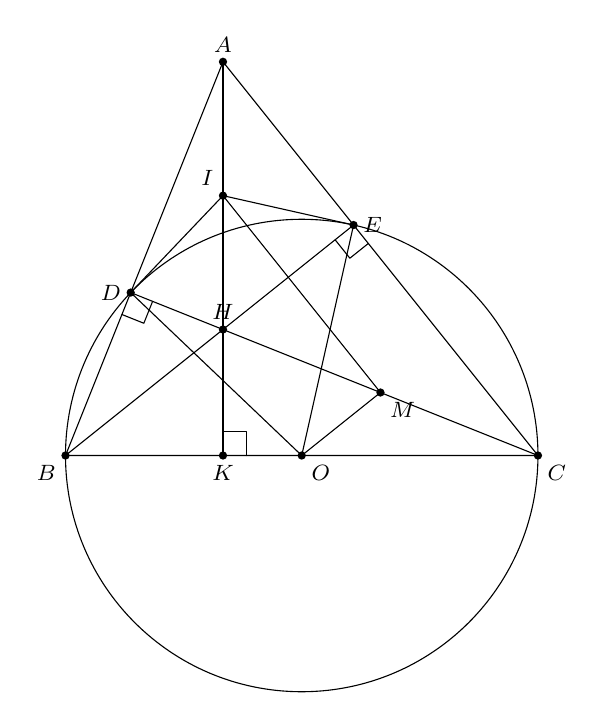
\begin{tikzpicture}[line join = round, line cap=round,>=stealth,font=\footnotesize,scale=1]
			\usetikzlibrary{calc,intersections,angles}
			
			% Khai báo hằng số
			\def\r{3} % r = 3cm
			
			% Định nghĩa tọa độ các điểm
			\coordinate (O) at (0,0);
			\coordinate (B) at (-\r,0); % B(-r;0)
			\coordinate (C) at (\r,0);  % C(r;0)
			\coordinate (A) at (-1,5); % A(-1;5)
			
			% D là hình chiếu của C lên AB
			\coordinate (D) at ($(A)!(C)!(B)$);
			% E là hình chiếu của B lên AC
			\coordinate (E) at ($(A)!(B)!(C)$);
			% K là hình chiếu của A lên BC (trục Ox)
			\coordinate (K) at ($(B)!(A)!(C)$); % Hoặc đơn giản là (A_x, 0) nếu BC là trục Ox, A_x là hoành độ của A
			
			% BE cắt CD tại H
			\path[name path=lineBE_H] (B) -- (E);
			\path[name path=lineCD_H] (C) -- (D);
			\path[name intersections={of=lineBE_H and lineCD_H, by=H}];
			
			% I là trung điểm của AH
			\coordinate (I) at ($(A)!0.5!(H)$);
			% M là trung điểm của HC
			\coordinate (M) at ($(H)!0.5!(C)$);
			
			% Vẽ các đối tượng hình học
			\draw (O) circle (\r);          % Đường tròn (O;r)
			\draw (A) -- (B) -- (C) -- cycle; % Tam giác A-B-C-A
			\draw (D) -- (I) -- (E) -- (O) -- cycle; % Đa giác D-I-E-O-D
			\draw (A) -- (K);               % Đoạn A-K
			\draw (B) -- (E);               % Đoạn B-E (đường cao)
			\draw (C) -- (D);               % Đoạn C-D (đường cao)
			\draw (O) -- (M) -- (I);        % Đường O-M-I
			
			% Tô màu cho các điểm (theo cấu trúc đầu tiên)
			\fill (O) circle (1.5pt);
			\fill (A) circle (1.5pt);
			\fill (B) circle (1.5pt);
			\fill (C) circle (1.5pt);
			\fill (D) circle (1.5pt);
			\fill (E) circle (1.5pt);
			\fill (H) circle (1.5pt);
			\fill (I) circle (1.5pt);
			\fill (M) circle (1.5pt);
			\fill (K) circle (1.5pt);
			
			% Đặt nhãn cho các điểm (theo cấu trúc đầu tiên)
			\node[below right] at (O) {$O$};
			\node[above] at (A) {$A$};
			\node[below left] at (B) {$B$};
			\node[below right] at (C) {$C$};
			\node[left] at (D) {$D$};       % Vị trí tương đối
			\node[right] at (E) {$E$};      % Vị trí tương đối
			\node[above] at (H) {$H$};      % Vị trí tương đối
			\node[above left] at (I) {$I$}; % Vị trí tương đối
			\node[below right] at (M) {$M$};% Vị trí tương đối
			\node[below] at (K) {$K$};      % Vị trí tương đối
			
			% Không có yêu cầu ký hiệu góc vuông trong lần này
			    \pic[draw, angle radius=3mm]{right angle = A--K--C};
			\pic[draw, angle radius=3mm]{right angle = B--D--C};
			\pic[draw, angle radius=3mm]{right angle = B--E--C};
		\end{tikzpicture}
		
	\end{center}
	}
\end{ex}

\setcounterref{ex}{0}
